\documentclass[11pt,a4paper]{article}
\usepackage[T1]{fontenc}
\usepackage[utf8]{inputenc}
\usepackage[english,portuguese]{babel}
\usepackage[margin=2.35cm]{geometry}
\usepackage{lmodern,microtype,booktabs,longtable,tabularx,array,graphicx,amsmath}
\usepackage[dvipsnames]{xcolor}
\usepackage{enumitem,fancyhdr,float,needspace}
\usepackage[numbers,sort&compress]{natbib}
\usepackage[colorlinks=true,linkcolor=MidnightBlue,citecolor=MidnightBlue,urlcolor=MidnightBlue,breaklinks=true]{hyperref}
\setlength{\parskip}{4pt}
\setlength{\parindent}{1em}
\setlist{nosep,leftmargin=*}
\renewcommand{\arraystretch}{1.18}
\setlength{\emergencystretch}{3em}
\pagestyle{fancy}\fancyhf{}
\fancyhead[L]{\small Revisão da integração IDS--SIEM}\fancyhead[R]{\small Síntese de 18 estudos}
\fancyfoot[C]{\thepage}\setlength{\headheight}{14pt}
\newcolumntype{P}[1]{>{\raggedright\arraybackslash}p{#1}}
\newcolumntype{Y}{>{\raggedright\arraybackslash}X}
\definecolor{ISCTEDarkBlue}{rgb}{0,0.08,0.45}
\newcommand{\instituicao}{Iscte -- Instituto Universitário de Lisboa}
\newcommand{\turma}{MEI A1}
\newcommand{\curso}{Mestrado em Engenharia Informática}
\newcommand{\autorUm}{Afonso Miguel Teixeira Januário}
\newcommand{\numeroUm}{146764}
\newcommand{\autorDois}{João Pedro Cravinho Dias}
\newcommand{\numeroDois}{145595}
\newcommand{\autorTres}{Sérgio Grubleac Silva}
\newcommand{\numeroTres}{144547}
\newcommand{\autorQuatro}{Wandir Etiene Louro Moreira de Castro}
\newcommand{\numeroQuatro}{137832}
\newcommand{\docente}{Valderi Reis Quietinho Leithardt}
\newcommand{\dataentrega}{Outubro de 2026}
\newcommand{\titulotrabalho}{Eficácia da integração entre IDS e SIEM na deteção de ataques em redes empresariais}
\newcommand{\subtitulotrabalho}{Segurança em Redes e Sistemas de Informação\\Revisão da literatura de âmbito delimitado}
\hypersetup{pdftitle={Eficácia da integração entre IDS e SIEM na deteção de ataques em redes empresariais},pdfauthor={Afonso Januário; João Dias; Sérgio Silva; Wandir Castro}}
\addto\captionsportuguese{\renewcommand{\contentsname}{Índice}\renewcommand{\listfigurename}{Índice de figuras}\renewcommand{\listtablename}{Índice de tabelas}}
\begin{document}
\hypersetup{pageanchor=false}
% Capa adaptada da primeira página de ambco-iscte/isctex (The Unlicense).
\newgeometry{margin=2.5cm}
\begin{titlepage}
\thispagestyle{empty}\sffamily\fontsize{14}{21}\selectfont
\setlength{\parskip}{0pt}\raggedright

\includegraphics[width=6.03cm]{imagens/iscte-pt.png}\par
\vspace{3.3mm}
{\color{ISCTEDarkBlue}\hrule height 0.4pt}
\vspace{1.3cm}
{\bfseries\titulotrabalho\par}
\subtitulotrabalho\par
\vspace{1.1cm}
\autorUm\ --- \numeroUm\par
\vspace{0.2cm}
\autorDois\ --- \numeroDois\par
\vspace{0.2cm}
\autorTres\ --- \numeroTres\par
\vspace{0.2cm}
\autorQuatro\ --- \numeroQuatro\par
\vspace{1.1cm}
\curso\par
Turma: \turma\par
\vspace{1.1cm}
Docente:\par
\vspace{0.4cm}
\docente\par
\instituicao\par
\vfill
\dataentrega\par
\end{titlepage}
\restoregeometry

\hypersetup{pageanchor=true}
\begin{abstract}
Esta revisão analisa a integração de IDS de rede com plataformas SIEM através de uma única pergunta de investigação. A síntese qualitativa integra 18 estudos e distingue centralização de alertas, combinação de sensores e correlação de contexto. A evidência indica viabilidade operacional e benefícios dependentes da configuração, mas não sustenta uma melhoria quantitativa universal face ao IDS isolado. As diferenças de comparadores, métricas e cenários limitam a atribuição dos ganhos ao SIEM. O trabalho adota um âmbito delimitado, com o percurso de seleção documentado no apêndice, e apresenta implicações para a avaliação experimental em laboratório.
\end{abstract}

\noindent\textbf{Palavras-chave:} IDS de rede; SIEM; correlação de eventos; deteção de ataques; revisão da literatura.

\clearpage
\begin{otherlanguage}{english}
\begin{abstract}
This review examines the integration of network intrusion detection systems (IDS) with security information and event management (SIEM) platforms through a single research question. The qualitative synthesis covers 18 studies and distinguishes alert centralisation, the combination of sensors, and the correlation of contextual information. The evidence indicates operational feasibility and configuration-dependent benefits, but does not support a universal quantitative improvement over a standalone IDS. Differences in comparators, metrics, and scenarios limit the attribution of gains to the SIEM. The review adopts a bounded scope, documents the selection process in an appendix, and discusses implications for experimental evaluation in a laboratory.
\end{abstract}
\noindent\textbf{Keywords:} network IDS; SIEM; event correlation; attack detection; literature review.
\end{otherlanguage}

\clearpage
\begingroup
\hypersetup{linkcolor=black}
\pdfbookmark[0]{\contentsname}{indice-geral}
{\renewcommand{\baselinestretch}{0.9}\small\tableofcontents}
\clearpage
\phantomsection
\addcontentsline{toc}{section}{\listfigurename}
\listoffigures
\clearpage
\phantomsection
\addcontentsline{toc}{section}{\listtablename}
\listoftables
\clearpage
\endgroup

\phantomsection
\section*{Lista de siglas e abreviaturas}
\addcontentsline{toc}{section}{Lista de siglas e abreviaturas}
\begin{description}[style=multiline,leftmargin=2.1cm,font=\normalfont\bfseries,itemsep=3pt]
\item[DDoS] Distributed Denial of Service: negação de serviço distribuída.
\item[DMZ] Demilitarized Zone: zona desmilitarizada da rede.
\item[DoS] Denial of Service: negação de serviço.
\item[FN] False Negative: falso negativo, ataque não detetado.
\item[FP] False Positive: falso positivo, atividade benigna classificada como ataque.
\item[FPR] False Positive Rate: taxa de falsos positivos, $FP/(FP+TN)$.
\item[IA] Inteligência artificial.
\item[IDS] Intrusion Detection System: sistema de deteção de intrusões.
\item[IoT] Internet of Things: Internet das Coisas.
\item[IPS] Intrusion Prevention System: sistema de prevenção de intrusões.
\item[LAN] Local Area Network: rede local.
\item[LLM] Large Language Model: modelo de linguagem de grande dimensão.
\item[NIDS] Network Intrusion Detection System: IDS baseado na análise da rede.
\item[NTA] Network Traffic Analysis: análise de tráfego de rede.
\item[OT] Operational Technology: tecnologia operacional.
\item[PCAP] Packet Capture: captura de pacotes de rede e respetivo formato de ficheiro.
\item[PI] Pergunta de investigação.
\item[PICOC] Population, Intervention, Comparison, Outcome, Context: população, intervenção, comparação, resultados e contexto.
\item[RAG] Retrieval-Augmented Generation: geração apoiada na recuperação de informação.
\item[SIEM] Security Information and Event Management: gestão de informação e eventos de segurança.
\item[SOC] Security Operations Center: centro de operações de segurança.
\item[TLS] Transport Layer Security: protocolo de proteção das comunicações.
\item[TN] True Negative: verdadeiro negativo, atividade benigna corretamente identificada.
\item[TP] True Positive: verdadeiro positivo, ataque corretamente detetado.
\item[VM] Virtual Machine: máquina virtual.
\end{description}
\clearpage

\section{Introdução}
\subsection{Enquadramento e motivação}
O projeto de grupo propõe um laboratório virtual com LAN, DMZ e zona de servidores, políticas de firewall, IDS/IPS e SIEM. Prevê ataques controlados de reconhecimento, força bruta e SQL injection, seguidos de endurecimento e repetição dos ensaios. Neste contexto, a revisão procura fundamentar uma decisão concreta: perceber o que a integração do IDS com o SIEM pode acrescentar à deteção e como avaliar esse contributo.

A literatura distingue recolha, normalização, correlação e apresentação dos eventos como funções de um SIEM \citep{gonzalez2021}. Estas capacidades permitem reunir informação dispersa e apoiar a análise de acontecimentos relacionados. Porém, receber alertas num painel central não significa necessariamente detetar ataques adicionais, reduzir falsos positivos ou produzir uma decisão mais cedo. A motivação do trabalho é compreender em que condições a integração traz benefícios e que evidência permite sustentá-los.

Esta distinção tem consequências para o laboratório. Se forem alterados simultaneamente os sensores, as regras e as fontes de dados, uma melhoria observada não pode ser atribuída apenas ao SIEM. A revisão ajuda, por isso, a separar o funcionamento da solução da avaliação do seu efeito e a escolher condições de comparação adequadas.

\subsection{Problema e pergunta de investigação}
O problema consiste em determinar se a evidência disponível permite distinguir o efeito da integração dos efeitos de outras alterações introduzidas nos sistemas avaliados. O interesse centra-se na identificação correta de ataques, considerando também falsos positivos e tempo de deteção. O trabalho mantém uma única pergunta:
\begin{quote}
\textbf{PI1: Que efeito tem a integração de um IDS de rede com uma plataforma SIEM na eficácia da deteção de ataques em redes empresariais, em comparação com a utilização isolada do IDS?}
\end{quote}
A análise não pressupõe um efeito favorável. Perda de informação ou aumento da latência também são resultados relevantes. Segmentação, endurecimento e tipos de ataque são variáveis de contexto, não perguntas adicionais.

\subsection{Objetivos e âmbito}
O objetivo geral é analisar criticamente a evidência sobre a contribuição da integração IDS--SIEM para a deteção de ataques, em comparação com a utilização isolada do IDS. Para o concretizar, definem-se quatro objetivos específicos:
\begin{enumerate}
\item Caracterizar as configurações, as fontes de eventos e os mecanismos de integração utilizados nos 18 estudos incluídos.
\item Comparar os desenhos de avaliação, as métricas e os resultados, identificando as condições que permitem ou impedem atribuir um efeito à integração.
\item Distinguir resultados de deteção, ganhos de processamento e demonstrações de funcionamento, explicitando as limitações da evidência.
\item Traduzir a síntese em orientações para a comparação experimental a realizar no laboratório do projeto.
\end{enumerate}

Esta entrega apresenta uma revisão da literatura de âmbito delimitado. A análise incide sobre os 18 estudos selecionados; as referências adicionais apoiam o enquadramento e a metodologia. Não foram executados os ensaios dos artigos nem a experiência proposta para o laboratório. As condições de seleção e as limitações de reprodução são descritas na metodologia e no apêndice.

\subsection{Contributos do trabalho}
O trabalho apresenta uma comparação estruturada dos 18 estudos, relacionando cada configuração com o comparador utilizado, o resultado principal e os limites da sua interpretação. A síntese permite separar três intervenções frequentemente associadas à integração: centralizar alertas, combinar sensores e correlacionar informação de diferentes fontes.

Outro contributo é a identificação das condições necessárias para avaliar o efeito da integração: manter comparáveis os cenários e as regras, definir a unidade de análise e reportar os denominadores das métricas. Estas condições sustentam a proposta de ensaios para o laboratório. O contributo é analítico e metodológico; não corresponde a uma nova ferramenta ou a uma melhoria de deteção demonstrada experimentalmente pelo grupo.

\section{Fundamentação teórica e trabalhos relacionados}
\subsection{O papel do IDS e do SIEM}
Um IDS de rede observa o tráfego disponível no ponto onde está instalado e produz alertas sobre atividades potencialmente maliciosas. O SIEM recebe eventos de diferentes origens e permite analisá-los em conjunto. As duas funções são complementares: o sensor fornece evidência sobre a comunicação e a plataforma reúne essa evidência com registos de sistemas, aplicações e outros dispositivos \citep{gonzalez2021}.

Um alerta do IDS não deve ser confundido com a confirmação de um incidente. O seu significado depende do comportamento observado, das regras e do contexto. Por exemplo, um alerta de exploração pode justificar investigação sem demonstrar que o ataque teve sucesso. Em I088, a associação entre eventos de rede e alterações num sistema ilustra a utilidade de combinar essas perspetivas para apoiar a auditoria \citep{ossimaudit2015}.

Também importa distinguir deteção de prevenção. Um IDS assinala atividade suspeita; uma função de prevenção acrescenta uma ação, como bloquear uma comunicação. Nesta revisão, resultados de bloqueio ou notificação são considerados indicadores complementares: não substituem a medição da capacidade de identificar corretamente os ataques.

\subsection{Da recolha à correlação de eventos}
A integração envolve mais do que enviar alertas para um painel. A arquitetura SIEM inclui recolha de eventos, tratamento de formatos, armazenamento e análise. Estes passos permitem trabalhar com dados produzidos por ferramentas diferentes, mas introduzem requisitos de configuração e de capacidade de processamento \citep{manzoor2024}.

A \textit{normalização} organiza campos heterogéneos numa representação comum. A \textit{agregação} reúne eventos relacionados ou repetidos. A \textit{correlação} aplica relações entre evidências, por exemplo através de endereços, instantes e sequências de ações. A revisão de \citet{kotenko2022} enquadra a diversidade destes métodos. Já I057 demonstra consultas comuns sobre registos de Snort e de outras fontes, sem medir um ganho de deteção face ao sensor isolado \citep{normalisation2014}.

Como exemplo ilustrativo, um alerta de rede pode ser relacionado com falhas de autenticação e um acesso posterior ao mesmo servidor. Essa combinação pode justificar uma prioridade diferente da atribuída a cada evento isolado. Porém, é necessário verificar se os endereços e os instantes correspondem à mesma atividade. Neste exemplo conceptual, a existência de uma regra de correlação não demonstra, por si só, que a decisão esteja correta.

\subsection{Centralização, contexto e contribuição efetiva}
Existem três alterações que convém separar: transportar os alertas do mesmo IDS para um SIEM, acrescentar outros sensores e introduzir novas regras ou fontes de contexto. Cada alteração responde a uma necessidade diferente e pode modificar os resultados. A comparação entre ferramentas SIEM apresentada por \citet{manzoor2024} ajuda a discutir capacidades e consumo de recursos, mas não estima automaticamente o benefício de integrar um IDS específico.

Os estudos incluídos mostram por que razão esta distinção importa. S041 permite comparar Snort isolado com ArcSight alimentado pelo mesmo Snort, enquanto A257 altera os registos dos sistemas Windows e as regras usadas na análise \citep{negi2021,uetz2021}. No segundo caso, um ganho pode resultar da informação adicional. Atribuí-lo apenas à presença do SIEM ocultaria uma parte essencial da intervenção.

Na leitura dos estudos, procuramos por isso identificar o que mudou, o que foi mantido e qual é a unidade avaliada. Um teste com ficheiros de tráfego, uma contagem de alarmes e um exercício realizado por analistas não medem necessariamente o mesmo efeito.

\subsection{Como interpretar a eficácia e o desempenho}
O \textit{recall} expressa a proporção de ataques de referência que foram detetados. A \textit{precisão} indica a proporção de deteções positivas que corresponde a ataques. O F1 combina ambas as medidas. A taxa de falsos positivos exige ainda uma definição dos casos benignos e do seu denominador. As fórmulas utilizadas são apresentadas na secção dedicada ao laboratório.

Estas medidas só são comparáveis quando as unidades também o são. Um único ataque pode gerar vários alertas; contar esses alertas como ataques independentes altera o significado dos resultados. Do mesmo modo, detetar pelo menos um evento em cada cenário não permite calcular a precisão sem conhecer as deteções incorretas. A distinção é relevante para interpretar a cobertura de sessões em P03 e os denominadores de S032 \citep{suryayusra2026,wazuhtelegram2026}.

O desempenho operacional constitui outra dimensão. Tempo de processamento, atraso de indexação, entrega de uma notificação e tempo até à deteção correta têm pontos de início e de fim diferentes. P02 compara a eficiência de motores de correlação; esses resultados são úteis para avaliar processamento, mas não equivalem a melhoria de recall \citep{sheeraz2024}. A revisão mantém estas dimensões separadas para responder à PI1 sem transformar resultados de funcionamento em conclusões causais sobre deteção.

\section{Metodologia}
\subsection{Protocolo e âmbito}
O protocolo fornecido pelo docente orienta a definição do problema, a pesquisa, a seleção e a extração. A estrutura foi adaptada à PI1. O PRISMA 2020 serve de referência para transparência do relato \citep{page2021}, sem alegar cumprimento integral.

Foram consultadas IEEE Xplore, ACM Digital Library e Scopus, complementadas por descoberta exploratória em páginas editoriais e repositórios. As pesquisas decorreram em 21 e 22 de outubro de 2026; a seleção focalizada foi revista em 24 de outubro de 2026. O Parsifal apoiou a gestão dos registos e decisões; os registos de pesquisa e extração foram conservados no repositório como documentação de trabalho. A síntese foi delimitada aos 18 estudos incluídos, com os detalhes do processo apresentados no Apêndice~\ref{app:metodo}.

Os resultados das bases não são diretamente comparáveis como medidas de rendimento: Scopus utilizou título/resumo/palavras-chave; a ACM pesquisou texto completo na coleção ACM, incluindo registos de volumes de atas. Os URLs históricos das consultas IEEE foram recuperados: preservam a expressão no parâmetro \texttt{queryText}, mas não um qualificador de campo. O campo efetivo não pôde, por isso, ser confirmado; esta limitação impede a reprodução exata da configuração histórica. Não se assume uma pesquisa exaustiva de toda a literatura.

A seleção e a extração foram preparadas com assistência de IA sem validação independente documentada. Não houve revisão independente por dois investigadores, cálculo de concordância ou execução dos experimentos dos artigos. As referências foram confrontadas com páginas editoriais, repositórios e/ou Crossref, preservando as dúvidas encontradas.

\Needspace{15\baselineskip}
\subsection{Disponibilidade dos resultados e documentação}
O relatório, as fontes LaTeX e os dados que sustentam a revisão estão disponíveis no repositório público \url{https://github.com/afonsojanu/srsi-ids-siem}. O repositório reúne a extração dos 18 estudos, as decisões de seleção, as contagens dos gráficos e os registos das pesquisas. Estes materiais permitem acompanhar a relação entre as fontes consultadas e a síntese apresentada. As exportações históricas mantêm as datas e as limitações descritas no apêndice. Os textos completos dos artigos não são redistribuídos; as referências bibliográficas identificam as fontes originais.

\subsection{PICOC}
\begin{table}[H]\centering\small
\begin{tabularx}{\linewidth}{@{}p{2.5cm}Y@{}}\toprule
Elemento & Definição operacional\\\midrule
População & Redes empresariais e laboratórios com serviços e tráfego aplicáveis a essas redes.\\
Intervenção & Integração operacional de NIDS e SIEM, incluindo alertas e, quando existente, correlação com outras fontes.\\
Comparação & Mesmo IDS sem correlação do SIEM, idealmente com tráfego, regras, hardware e topologia equivalentes.\\
Resultados & Recall, precisão, F1, taxa de falsos positivos e tempo de deteção. Cobertura de cenários, volume de alertas e custo computacional são complementares.\\
Contexto & Avaliações empíricas com ataques identificados. Aplicações exclusivamente IoT especializadas exigem demonstração de aplicabilidade empresarial.\\\bottomrule
\end{tabularx}\caption{Delimitação da única pergunta de investigação.}\end{table}

\subsection{Estratégia de pesquisa}
Os grupos conceptuais são IDS, SIEM e integração/correlação. A expressão principal utilizada foi:
\begin{quote}\small\ttfamily\raggedright
("intrusion detection system" OR "network intrusion detection" OR IDS OR NIDS)\\
AND ("security information and event management" OR SIEM)\\
AND (integration OR correlation OR "event correlation" OR "alert correlation" OR "log correlation")
\end{quote}
Para localizar revisões relacionadas, acrescenta-se:
\begin{quote}\small\ttfamily\raggedright
AND ("systematic literature review" OR "systematic review" OR "literature review" OR survey)
\end{quote}
As consultas complementares utilizaram nomes de ferramentas e procuraram versões públicas dos textos. A execução e as sobreposições com a pesquisa principal estão documentadas no apêndice metodológico.

As revisões de \citet{gonzalez2021} e \citet{kotenko2022} ajudam a delimitar o problema: a primeira enquadra as funções do SIEM e a segunda organiza métodos de correlação de eventos. Nesta revisão, essa distinção orienta a análise da integração operacional e dos comparadores, evitando tratar qualquer uso de SIEM como prova de melhoria. Na conferência de 30 de outubro, manteve-se a expressão por grupos IDS, SIEM e integração/correlação. Esta fundamentação documenta a adequação da expressão ao âmbito escolhido; não altera a ordem histórica das pesquisas nem equivale a uma validação da sua sensibilidade.

O limite temporal é 21 de outubro de 2026, sem ano inicial obrigatório; os idiomas são inglês e português. As pesquisas principais não aplicaram limite inferior de ano; os idiomas foram tratados na seleção. A reprodução exata depende dos campos efetivos de cada interface, cuja documentação tem as limitações explicitadas nesta revisão. A pesquisa por referências foi identificada como via complementar. O registo de trabalho inclui consultas de descoberta e de recuperação, identificando a primeira localização de cada candidato; não mede o total de resultados do motor.

\subsection{Elegibilidade}
Incluem-se artigos de revistas ou conferências com revisão por pares, em inglês/português, com integração concreta NIDS--SIEM, avaliação empírica e contexto aplicável à PI1. O comparador direto não é obrigatório para a síntese descritiva, mas é indispensável para estimar o efeito incremental. A seleção focalizada aplica ainda R1 (pontuação inferior a 3,5/6) e R2 (experiência centrada apenas na captura/processamento do sensor, sem avaliar o contributo da cadeia SIEM). A alteração posterior dos critérios e as decisões individuais constam do apêndice.
\begin{table}[H]\centering\small
\begin{tabularx}{\linewidth}{@{}P{1.2cm}Y@{}}\toprule
Código & Motivo principal de exclusão\\\midrule
E1 & Tipo de publicação/revisão por pares incompatível ou não confirmado: tese, poster ou preprint sem versão revista identificada.\\
E2 & Não avalia a integração operacional de NIDS e SIEM, ou não apresenta avaliação empírica pertinente.\\
E3 & Contexto especializado sem aplicabilidade demonstrada à população definida.\\
E4 & Idioma fora do âmbito.\\
E5 & Estudo secundário, reservado ao enquadramento e à identificação de referências.\\
E6 & Duplicado ou versão do mesmo estudo sem informação adicional.\\\bottomrule
\end{tabularx}\caption{Critérios de exclusão. Regista-se um motivo principal por decisão.}\end{table}
A ausência de avaliação integral não constitui prova de irrelevância. Os registos fora da avaliação delimitada são distinguidos das exclusões por critérios de elegibilidade no apêndice.

\subsection{Seleção e extração}
O processo compreende importação, deduplicação global por DOI/título normalizado, triagem por título/palavras-chave, leitura de resumo e decisão por texto completo. Preservou-se a ficha exploratória quando já continha notas; entre as novas bases, a precedência foi IEEE, ACM e Scopus. As contagens por fonte após deduplicação refletem esta atribuição, não amostras independentes. As três passagens de \citet{keshav2007} orientam a compreensão global, a leitura dos métodos/resultados e a avaliação crítica. A referência original é de 2007, volume 37(3), páginas 83--84, corrigindo a indicação incompleta presente no protocolo fornecido.

A extração regista identificador, referência, acesso, configuração, fontes e mecanismos de integração, ataques, comparador, métricas, resultados, limitações e localização da evidência. A extração da síntese focalizada contém 18 fichas e dez campos por estudo (180 campos), preenchidos no Parsifal. A tabela comparativa e a análise dos estudos apresentam os resultados desta extração. As fichas da avaliação anterior são conservadas para auditoria; a nova seleção não apaga a evidência já extraída. Distingue-se informação não reportada pelo artigo de pormenores não recuperados na ficha consolidada, nomeadamente algumas versões das ferramentas; nenhum destes casos é convertido em zero. As observações dos artigos são distinguidas das interpretações desta revisão.

A força da evidência é classificada em \textbf{A}: comparação que isola a integração; \textbf{B}: comparação entre variantes de SIEM, motores ou arquiteturas; \textbf{C}: demonstração sem comparador. Classes B/C podem ser tecnicamente úteis sem permitir resposta causal à PI1.

\subsection{Qualidade e síntese}
Avaliam-se seis dimensões: Q1, configuração; Q2, ataques e referência de verdade; Q3, comparador que isola a integração; Q4, tráfego benigno e denominadores; Q5, repetibilidade e dados; Q6, limitações. Atribui-se 1 (suficiente), 0,5 (parcial) ou 0 (não demonstrado). São itens metodológicos, não novas perguntas de investigação. Na reformulação de 24 de outubro de 2026, adotou-se um limiar de 3,5/6 para a síntese focalizada, juntamente com a pertinência do objeto avaliado. Esta decisão foi posterior à leitura e não fazia parte do protocolo inicial; constitui uma limitação de seleção, não uma escala validada de risco de viés. Em 30 de outubro, alinhou-se o filtro automático do Parsifal com este limiar: como a plataforma aplica uma comparação estritamente superior, configurou-se o corte em 3,0. Na escala de meio ponto utilizada, pontuação superior a 3,0 equivale a pontuação igual ou superior a 3,5. Não se alteraram respostas, pontuações ou os 18 estudos aceites.

A inclusão tem uma interpretação funcional: abrange NIPS/NTA e plataformas que centralizam alertas de rede, mesmo quando não isolam a correlação do SIEM. A aplicação funcional a NTA e a laboratórios OT é assinalada como limite de generalização; não se trata todos os estudos como comparações causais equivalentes.

A síntese é narrativa. Não se realiza meta-análise porque os comparadores, as unidades e os indicadores não são equivalentes. Os perfis de qualidade acompanham a interpretação, sem tratar a soma como escala validada.

\section{Síntese dos 18 estudos}
O corpus final reúne \textbf{18 estudos}. A seleção dá prioridade à informação metodológica disponível, preservando resultados favoráveis, nulos e desfavoráveis à integração. As referências de enquadramento e de metodologia não são contadas como estudos incluídos.
\begin{figure}[H]\centering
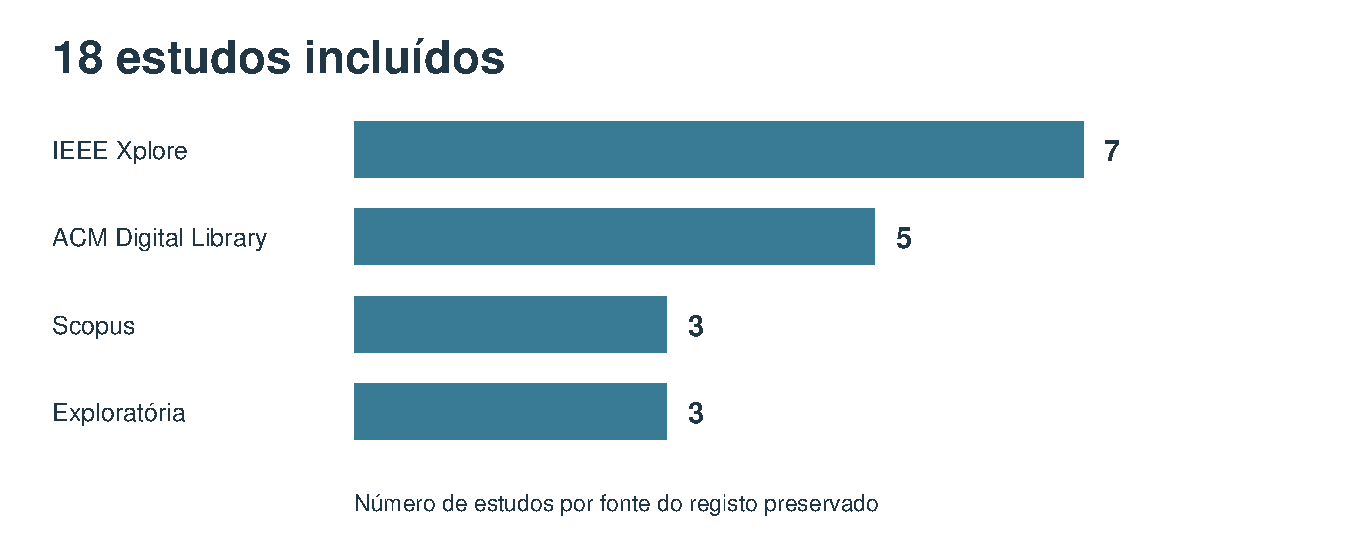
\includegraphics[width=.88\linewidth]{figures/estudos-incluidos.pdf}
\caption[Estudos incluídos por fonte do registo preservado]{Estudos incluídos por fonte do registo preservado. Contagem única após deduplicação e seleção focalizada; figura elaborada a partir dos registos da revisão.}\label{fig:incluidos}
\end{figure}
\subsection{Comparação dos estudos incluídos}
A Tabela~\ref{tab:comparacao-estudos} reúne a configuração, o comparador e o resultado principal de cada estudo. A ordem acompanha os grupos da síntese detalhada. Os valores são reportados pelos autores, salvo indicação de recálculo nesta revisão; não constituem resultados de experiências realizadas pelo grupo. A tabela não estabelece uma classificação de ferramentas, pois as tarefas e as métricas diferem entre estudos.

\begingroup\small
\setlength{\tabcolsep}{4pt}
\renewcommand{\arraystretch}{1.14}
\begin{longtable}{@{}P{1.15cm}P{2.65cm}P{3.0cm}P{3.5cm}P{4.85cm}@{}}
\caption[Comparação dos 18 estudos incluídos]{Comparação dos 18 estudos: configuração, comparação realizada, resultado principal e limite de interpretação.}\label{tab:comparacao-estudos}\\
\toprule Estudo & Configuração & Comparador ou desenho & Resultado principal & Limite de interpretação\\\midrule
\endfirsthead
\multicolumn{5}{l}{\textit{Tabela \thetable{} -- continuação}}\\
\toprule Estudo & Configuração & Comparador ou desenho & Resultado principal & Limite de interpretação\\\midrule
\endhead
\midrule\multicolumn{5}{r}{\textit{Continua na página seguinte.}}\\\endfoot
\bottomrule\endlastfoot
S041\newline\citep{negi2021} & Snort, Suricata e Bro / ArcSight & Mesmo Snort isolado e integrado; combinação de sensores. & 9/11 PCAPs em ambos os casos com Snort; 11/11 ao combinar sensores. & Sensores adicionais impedem atribuir o ganho apenas ao SIEM.\\[5pt]
P05\newline\citep{maliki2024} & Snort, Zeek e Suricata / Wazuh & Sensores individuais versus concordância dos três. & Snort: 95,4\%; correlação: 84,0\%, recalculados da tabela. & O artigo também refere 84,1\% e 84,6\%; sem denominador benigno.\\[5pt]
I063\newline\citep{hybridalarms2019} & Snort / Prelude; contexto Nessus & Alarmes antes e depois da priorização. & Redução de 77,9\% no volume com limiar de prioridade 1,5. & Reduzir alarmes não prova melhor deteção; pode despromover alarmes verdadeiros.\\[5pt]
S076\newline\citep{bryant2020} & Snort / SIEM com classificação por kill chain & Configuração base versus modificada. & 7/26 para 25/26 casos; 83 para 46 alertas. & Regras e ontologia mudam em conjunto; sem IDS isolado.\\[5pt]
I036\newline\citep{otrobustness2026} & IDS multicamada / SIEM em OT & Duas campanhas de 25 execuções. & 151/208 para 204/220 ações detetadas. & Mudam regras e percurso do ataque; sem isolamento do efeito do SIEM.\\[5pt]
A058\newline\citep{saibersoc2022} & Suricata / Security Onion & Configurações de regras avaliadas por analistas. & 19/73 e 29/89 relatórios identificam ataques injetados. & Mede identificação por analistas; inconsistência na distribuição dos grupos.\\[5pt]
A257\newline\citep{uetz2021} & Suricata / ELK; logs Windows & Configuração de logging base versus detalhada. & 4/9 para 6/9 passos; 40 execuções. & Ganho associado a logs de host; análise após exportação, sem IDS isolado.\\[5pt]
A052\newline\citep{roelofs2024} & NTA / plataforma multissistema & XGBoost versus regras sobre as mesmas fontes. & No teste temporal, identifica 2 dos 4 dias positivos. & Validação com SMOTE antes da divisão; dados privados e poucos dias positivos.\\[5pt]
A146\newline\citep{ragincident2026} & Suricata / Security Onion e RAG & Fontes e modelos de investigação distintos. & Recall médio de respostas: 94\% e 89\%, conforme o modelo. & Mede recuperação forense, não deteção de ataques; variam fontes e modelos.\\[5pt]
P02\newline\citep{sheeraz2024} & Snort / CTMS; motores OC e SEC & Comparação entre motores de correlação. & Ganhos reportados de cerca de 21 vezes em tempo real e 2,5 em CPU. & Eficiência de processamento; apenas duas regras, sem efeito isolado na deteção.\\[5pt]
P03\newline\citep{suryayusra2026} & Suricata / Wazuh & Sem condição equivalente de IDS isolado. & 60/60 sessões acionam uma regra; 25 414 eventos. & Cobertura de cenários; sem controlo benigno para estimar precisão.\\[5pt]
S032\newline\citep{wazuhtelegram2026} & Suricata / Wazuh e Telegram & Sem IDS isolado; seis classes de ataque. & Recall 0,83--0,97; precisão 0,89--1,00. & Unidades misturam alertas e intervalos; notificação não é deteção.\\[5pt]
I010\newline\citep{chandran2026} & Detetor de portscan / Splunk & Sem comparação com e sem SIEM. & Recall 89\%; precisão 96,74\%; F1 92,71\%, recalculados. & 200 casos de ataque e 10 000 benignos; efeito da integração não isolado.\\[5pt]
I014\newline\citep{pattinama2026} & SLIPS / Filebeat e ELK & Demonstração sem comparador. & Latências reportadas de 6, 18 e 3 s; média de 9 s. & Instantes medidos no SLIPS; não medem o percurso completo até ao SIEM.\\[5pt]
I024\newline\citep{predictive2026} & Random Forest / Wazuh & Avaliação do classificador integrado. & Accuracy 92,34\%; precisão de 60\% na classe Infiltration. & Sem condição sem Wazuh; partição e pré-processamento parcialmente descritos.\\[5pt]
I057\newline\citep{normalisation2014} & Snort e outras fontes / OLF-UERM & Demonstração de normalização e consulta. & 260 336 linhas no conjunto HN34. & Sem recall, FPR ou ganho medido face a Snort isolado.\\[5pt]
I088\newline\citep{ossimaudit2015} & Snort, Suricata e OSSEC / OSSIM & Demonstração de auditoria em laboratório. & Relaciona eventos de rede e de host em cenários de ataque. & Alguns passos não observados; sem matriz de confusão ou IDS isolado.\\[5pt]
A012\newline\citep{ctismes2025} & Suricata / Graylog e MISP & Emulação de dez técnicas, sem comparador. & 14 alertas no download e nove na persistência. & Demonstra funcionamento e contexto; sem eficácia incremental quantificada.\\[5pt]
\end{longtable}
\endgroup

A comparação evidencia que a existência de uma integração funcional é mais frequente do que a avaliação do seu efeito isolado. S041 oferece um contraste limitado com o mesmo sensor e I063 analisa a priorização dos mesmos alarmes. Os restantes desenhos alteram configurações, fontes ou modelos, ou demonstram uma cadeia integrada sem condição de controlo. Por isso, os benefícios observados devem ser associados ao que cada experiência realmente modificou.

\subsection{Comparação direta limitada e efeitos da correlação}
\paragraph{S041.} \citet{negi2021}: Integram Snort 3, Suricata e Bro no ArcSight, com conectores, normalização e regras de correlação por endereços IP. A tabela 1 contém 11 PCAPs: Snort e ArcSight alimentado apenas por Snort identificam os mesmos nove; Suricata identifica oito e Bro cinco. A combinação tem pelo menos um sensor positivo em todos os 11. Estas contagens foram recalculadas da tabela original; os valores 1--3 da coluna combinada representam concordância dos sensores, não probabilidades de deteção. A comparação com o mesmo Snort é um indício limitado de efeito nulo na cobertura desses ficheiros. A diferença de 9/11 para 11/11 envolve acrescentar sensores, pelo que não isola o efeito do SIEM. Não há quantificação de FP/TN, repetições ou intervalos de confiança.

\paragraph{P05.} \citet{maliki2024}: Avaliam SYN flood em cinco ensaios de 100 ataques por IDS. A tabela I apresenta médias de deteção de 95,4\% para Snort e 88,6\% para Zeek e Suricata. A média da coluna de correlação, calculada nesta revisão a partir de 88, 75, 87, 83 e 87, é 84,0\%. O corpo do artigo refere 84,1\%, enquanto resumo e conclusão referem 84,6\%: conserva-se explicitamente esta inconsistência. A correlação exige concordância dos três sensores. O resultado não demonstra melhoria face a Snort nem permite estimar FPR sem denominador benigno.

\paragraph{I063.} \citet{hybridalarms2019}: Snort envia alarmes em IDMEF ao Prelude, que usa perfis de vulnerabilidades Nessus para priorização. O filtro por IP reduz 2985 alarmes a 1858 (37,8\%); o limiar de prioridade de 1,5 reduz o volume em 77,9\%. Os autores reportam 75\% de deteção, 100\% de precisão e 25\% de falsos negativos na atribuição de prioridade. Estas medidas não são recall de ataques nem FPR sobre tráfego benigno. Inconsistências de versões e vulnerabilidades podem despromover alarmes verdadeiros. A comparação antes/depois apoia a análise de triagem, mas não demonstra que eliminar mais alarmes melhora a deteção. Classe A, limitada à priorização.

\paragraph{S076.} \citet{bryant2020}: Nos 26 casos, a configuração base deteta 7/26 e a modificada 25/26 (26,9\% e 96,2\%; diferença de 69,2 pontos percentuais). A tabela 2 mostra 83 versus 46 alertas; o scan SMB falha em ambas. O comparador é SIEM base, não Snort isolado. As regras e a ontologia mudam conjuntamente (128 versus 39 regras). A redução de alertas fora dos testes não fornece FPR com denominador benigno nem validação independente; médias de 100/dia e 1/dia não tornam os totais 2364 e oito diretamente comparáveis. Tempo de deteção e esforço são inferidos, não medidos. B: comparação de configurações do mesmo SIEM.

\paragraph{I036.} \citet{otrobustness2026}: Realizam duas campanhas de 25 execuções num laboratório Modbus. A deteção passa de 151/208 ações (72,6\%) para 204/220 (92,7\%) após introdução de quatro regras SIEM. A alteração simultânea da extração de credenciais e do número de ações impede atribuir toda a diferença apenas às regras. Não há comparação com IDS isolado. A latência inicial tem mediana de 9,6 s e percentil 95 de 42,8 s. Reportam zero falsos positivos em 50 minutos benignos, mas o algoritmo indica um minuto por execução e o texto dois minutos. A referência de verdade provém do CALDERA; o emparelhamento temporal condiciona a atribuição das deteções OT. Classe B.

\subsection{Fontes adicionais, configuração e investigação de incidentes}
\paragraph{A058.} \citet{saibersoc2022}: Compara regras Suricata predefinidas com remoção de 2753 regras de política, mantendo deteções dos ataques Mirai/Exim. 63 grupos, 162 relatórios; 19/73 e 29/89 relatórios identificam ataques injetados. OR reportado para Exim=3,04, p=0,03. Mede identificação por analistas; não compara IDS isolado. O texto inverte a atribuição de 31/32 grupos entre métodos e resultados e apresenta inconsistência na soma de participantes. A085 relata o mesmo experimento e foi excluído para evitar contagem dupla. B: comparação de configurações do SOC.

\paragraph{A257.} \citet{uetz2021}: Quarenta execuções: dez por configuração em dois computadores. Configuração Windows predefinida deteta quatro dos nove passos; configuração com Sysmon e PowerShell detalhado deteta seis, em todas as execuções. Os alertas Suricata mantêm-se; ganho vem dos logs de host e regras Sigma aplicadas após exportação do Elasticsearch. Não compara IDS isolado com SIEM nem mede correlação em tempo real. Alertas falsos/irrelevantes foram descartados antes da análise, impedindo inferir FPR. Artefactos públicos e repetição sustentam a análise de configuração. B: comparação de configurações de logging.

\paragraph{A052.} \citet{roelofs2024}: Empresa com mais de 50000 trabalhadores. Validação após SMOTE: TP = 592, FP = 2, TN = 11 121, FN = 0 e MCC = 0,998; o oversampling precede a divisão treino/validação, criando risco de dependência. No teste temporal independente há apenas quatro dias positivos de um mesmo exercício; deteta dois, após não detetar os dias de reconhecimento. Não são 592 ataques reais independentes. Compara XGBoost com regras sobre as mesmas fontes, não NIDS isolado. Dados e marcas privados limitam reprodução e atribuição do efeito ao SIEM. B/C: integração multissistema, sem IDS isolado.

\paragraph{A146.} \citet{ragincident2026}: 17 cenários, 94 948 eventos, 129 perguntas, 218 indicadores. Recall médio de respostas: 94\% Claude e 89\% DeepSeek. No cenário Fake Authenticator, Suricata-only fornece 40\% recall, enquanto RAG com fontes adicionais chega a 100\% em dois modelos. Mede recuperação de informação forense, não taxa de deteção de ataques; fontes, extração e raciocínio mudam simultaneamente. Cenário AD: 25/26 passos recuperados nos melhores modelos, precisão reportada 100\%. Consultas adaptadas aos cenários e ausência de controlo IDS/SIEM isolado limitam causalidade. B: comparação de fontes e modelos, com fatores adicionais.

\subsection{Cobertura, desempenho e viabilidade operacional}
\paragraph{P02.} \citet{sheeraz2024}: Comparam OC com SEC e demonstram correlação de eventos de Snort com registos de sistemas. Reportam ganhos de processamento de cerca de 21 vezes em tempo real e 2,5 vezes em tempo de CPU. O ensaio usa quatro tamanhos de ficheiro, duas regras e cinco execuções por tamanho. São medidas de eficiência de motores; não equivalem a redução de falsos positivos nem a melhoria de recall face ao IDS isolado.

\paragraph{P03.} \citet{suryayusra2026}: Apresentam 60 sessões de cinco categorias de ataque em 12 dias e 25 414 eventos centralizados. Todas as sessões acionaram pelo menos uma regra. Os autores distinguem cobertura de cenários de precisão e reconhecem ausência de controlo benigno. Não existe braço equivalente com IDS isolado. A referência adota o DOI e o mês da página editorial; a divergência com o cabeçalho do PDF é registada na nota bibliográfica. A evidência é funcional, não causal.

\paragraph{S032.} \citet{wazuhtelegram2026}: Seis classes de ataque durante 24 h. Tabela 2 fornece TP/FP/FN e recall 0,83--0,97, precisão 0,89--1,00. Definição mistura alertas (TP) com intervalos de ataque (FN), exigindo cautela no denominador. Tabela 3 reporta 0 FP em três demonstrações e atrasos Telegram 0,094/0,983/0,102 s; não generalizar 0 FP aos ensaios da tabela 2. Valores Splunk são citados de outra fonte, não comparação controlada. Sem baseline Suricata isolado; notificação não é tempo total de deteção. C: avaliação sem IDS isolado.

\paragraph{I010.} \citet{chandran2026}: Definem regras temporais de oito portas em 5 s, 15 ligações em 30 s e dez portas consecutivas em 8 s. A tabela I apresenta TP = 178, FN = 22, FP = 6 e TN = 9994: 200 casos de ataque e 10 000 benignos. Estes valores correspondem a accuracy de 99,73\%, precisão de 96,74\%, recall de 89\% e F1 de aproximadamente 92,71\%. A elevada accuracy reflete também o desequilíbrio da amostra. Reportam 15 000 pacotes/s, latência inferior a 250 ms e 88\% dos bloqueios em menos de 3 s. Não comparam o mesmo detetor com e sem Splunk; as métricas não isolam o efeito da integração. Classe C.

\paragraph{I014.} \citet{pattinama2026}: Utilizam SLIPS 2.0.3 para gerar alertas de varrimento de portas, força bruta SSH e DoS, enviados por Filebeat para ELK. Reportam latências de 6, 18 e 3 s, com média de 9 s, calculadas entre StartTime e CreateTime no SLIPS. Esta medida difere da latência entre alerta e indexação no SIEM definida na metodologia. O evento apresentado como DoS é uma ligação privada com nível Info, sem classificação inequívoca de DoS. Os recursos são amostrados a cada 5 s durante 25 minutos; o tráfego benigno usa um servidor separado e não há matriz de confusão. Não é isolado o benefício do SIEM. Classe C.

\paragraph{I024.} \citet{predictive2026}: Descrevem 51 atributos, 50 árvores RF e 1 000 107 amostras CICIDS, incluindo 200 022 no teste, com accuracy de 92,34\%. A classe Infiltration apresenta precisão de 60\%, apesar de classes volumétricas atingirem 1,00. A cadeia processa mais de 1000 fluxos/s e reporta menos de 100 ms por lote de 100; esta medida não equivale ao tempo até à deteção de um ataque. São métricas do classificador, sem comparação com e sem Wazuh. A precisão global superior a 92\% não define a taxa de falsos positivos. A sequência de pré-processamento e partição é parcialmente documentada. Classe C.

\paragraph{I057.} \citet{normalisation2014}: Analisam o conjunto HN34, com 260 336 linhas, incluindo 69 039 de Snort e 179 752 de IPtables, segundo a tabela II. A normalização OLF/UERM permite consultas comuns sobre múltiplas fontes; são apresentados exemplos SSH, SMTP e HTTP. Não são medidos recall, FPR ou ganho face a Snort isolado. O desempenho da normalização não equivale a eficácia de deteção. Classe C.

\paragraph{I088.} \citet{ossimaudit2015}: O OSSIM integra Snort, Suricata e OSSEC num laboratório com Windows 7 e Metasploitable. São demonstrados acesso a domínio malicioso, exploração seguida de alteração do grupo de administradores e túnel DNS. A ligação de eventos de rede e de host acrescenta contexto à auditoria; alguns passos não são observados. Não se apresentam IDS isolado, matriz de confusão ou estimativa de eficácia incremental. Classe C.

\paragraph{A012.} \citet{ctismes2025}: Emula Operation Sharpshooter com Caldera, dez técnicas em sete táticas. Suricata deteta RAT/C2; Graylog agrega alertas e contexto MISP, incluindo 14 alertas no download e nove na persistência. Demonstra contexto e funcionamento; não apresenta baseline IDS isolado, matriz de confusão ou repetição suficiente para eficácia incremental. Configuração e manutenção exigem esforço especializado. C: demonstração sem comparador.

\subsection{Qualidade e interpretação}
As pontuações apoiam a transparência da seleção e não demonstram ausência de viés. Um estudo pode obter uma pontuação relativamente elevada e continuar sem comparador IDS isolado. A inferência depende sobretudo do desenho experimental e dos denominadores, não apenas da soma.
\begin{longtable}{@{}lrrrrrrr@{}}\toprule
Estudo & Q1 & Q2 & Q3 & Q4 & Q5 & Q6 & Total\\\midrule\endhead
P02 & 1 & 1 & 0 & 0 & 1 & 1 & 4\\
P03 & 1 & 1 & 0 & 0 & 0,5 & 1 & 3,5\\
P05 & 1 & 1 & 0 & 0 & 0,5 & 1 & 3,5\\
A012 & 1 & 1 & 0 & 0 & 0,5 & 1 & 3,5\\
A052 & 0,5 & 1 & 0 & 1 & 0,5 & 1 & 4,0\\
A058 & 1 & 1 & 0 & 0,5 & 1 & 1 & 4,5\\
A146 & 1 & 1 & 0,5 & 0,5 & 1 & 1 & 5,0\\
A257 & 1 & 1 & 0 & 0 & 1 & 1 & 4\\
S032 & 1 & 1 & 0 & 0,5 & 0,5 & 0,5 & 3,5\\
S041 & 1 & 0,5 & 0,5 & 0,5 & 0,5 & 0,5 & 3,5\\
S076 & 1 & 1 & 0 & 0,5 & 0,5 & 0,5 & 3,5\\
I010 & 0,5 & 0,5 & 0 & 1 & 0,5 & 1 & 3,5\\
I014 & 1 & 1 & 0 & 0,5 & 0,5 & 1 & 4,0\\
I024 & 1 & 1 & 0 & 0,5 & 0,5 & 1 & 4,0\\
I036 & 1 & 1 & 0 & 0,5 & 0,5 & 1 & 4,0\\
I057 & 1 & 0,5 & 0 & 0 & 1 & 1 & 3,5\\
I063 & 1 & 1 & 0,5 & 0,5 & 0,5 & 1 & 4,5\\
I088 & 1 & 1 & 0 & 0 & 0,5 & 1 & 3,5\\
\bottomrule\caption{Avaliação dos 18 incluídos; justificações preservadas nas fichas.}\end{longtable}
\section{Discussão e resposta à PI1}
\textbf{A integração permite centralizar e relacionar evidências; o seu benefício incremental depende das fontes e das regras, e a evidência analisada ainda não permite estimar uma magnitude generalizável.} Esta resposta limita-se ao corpus analisado. S041 mostra cobertura inalterada ao ligar o mesmo Snort ao ArcSight, mas cobertura superior ao combinar sensores distintos. P05 mostra que uma regra de concordância pode perder cobertura face ao sensor mais sensível. I063 acrescenta uma comparação antes/depois de priorização no Snort--Prelude, com redução do volume e perda de prioridade de alguns alarmes verdadeiros. Nenhum destes resultados deve ser extrapolado para todas as redes ou ataques.

O potencial depende do que se acrescenta. Um SIEM que apenas reproduz alertas pode manter a contagem de ataques detetados. Fontes independentes e regras de correlação podem produzir decisões que um sensor sozinho não fornece. Trata-se de uma hipótese operacional coerente com os mecanismos descritos, não de uma magnitude demonstrada.

Devem distinguir-se visibilidade, qualidade da decisão e custo operacional. Um motor mais rápido não prova maior recall; uma notificação entregue não mede o momento de reconhecimento correto do ataque. A soma de alertas também não fornece o denominador de FPR. Um ataque pode produzir centenas de alertas verdadeiros redundantes. Agregá-los pode reduzir esforço sem alterar decisões erradas; uma queda nos alertas pode ainda resultar da perda de registos. É necessário medir qualidade e integridade da recolha em conjunto.

\section{Trabalhos futuros e implicações para o laboratório}
O laboratório pode responder à lacuna mantendo constante o IDS e separando integração de endurecimento. Propõem-se três condições, ainda não executadas:
\begin{table}[H]\centering\small
\begin{tabularx}{\linewidth}{@{}P{1.3cm}Y Y@{}}\toprule
Ensaio & Configuração & Interpretação\\\midrule
A & IDS com regras fixas, sem decisão de correlação do SIEM & Referência principal.\\
B & Mesmo IDS; SIEM recebe apenas os seus alertas & Consequências de centralização/transporte.\\
C & Mesmo IDS; SIEM correlaciona também logs de firewall e servidores & Efeito do pacote de integração e fontes adicionais face a A.\\\bottomrule
\end{tabularx}\caption{B distingue centralização de correlação; C não isola apenas o algoritmo do SIEM.}\end{table}

Manter topologia, recursos, ataques e tráfego benigno constantes; conservar versões e hashes das regras; sincronizar relógios; evitar contenção desigual de recursos. Reproduzir o mesmo tráfego quando possível e usar logs alinhados temporalmente. Afinar as regras em ensaios separados da avaliação.

Definir previamente a unidade: episódios de ataque identificados e janelas benignas de duração fixa, por exemplo. Fixar a janela máxima de associação do alerta ao episódio. Múltiplos alertas do mesmo episódio não contam como múltiplos ataques. As métricas são:
\begin{align*}
\mathrm{Recall}&=\frac{TP}{TP+FN}, &\mathrm{Precisão}&=\frac{TP}{TP+FP},\\
F_1&=\frac{2TP}{2TP+FP+FN}, &\mathrm{FPR}&=\frac{FP}{FP+TN}.
\end{align*}
Reportar os denominadores e a definição de TN. Quando TN não puder ser definido de forma defensável, usar também falsos alertas por hora de tráfego benigno, sem chamar FPR a essa frequência. Apresentar diferenças de recall em pontos percentuais, números absolutos e incerteza apropriada ao número de ensaios.

Medir o tempo entre o início conhecido do episódio e o primeiro alerta corretamente associado. Contar separadamente episódios não detetados, em vez de os omitir da análise. Distinguir latência do sensor, ingestão e correlação. Resposta humana exige um procedimento de observação próprio.

Executar a fase de endurecimento separadamente, identificando cada alteração. TLS e regras de firewall podem alterar a visibilidade ou impedir a ocorrência do ataque; esses efeitos não devem ser atribuídos à integração. O mapeamento ATT\&CK deverá descrever os cenários realmente executados e ser validado na versão utilizada pelo grupo.

\section{Limitações}
A revisão tem âmbito delimitado: os 18 estudos incluídos foram selecionados por critérios revistos de pertinência e qualidade e não constituem uma amostra aleatória nem uma cobertura exaustiva da literatura. O apêndice documenta a extensão da avaliação e distingue inelegibilidade de ausência de avaliação integral. As diferenças entre campos de pesquisa, as limitações da captura secundária ACM e as restrições de idioma e tipo de publicação condicionam a abrangência.

O limiar de qualidade e a delimitação focalizada foram definidos após a avaliação inicial, em resposta à redução do âmbito académico; esta seleção posterior pode introduzir viés e não representa um protocolo integralmente pré-especificado. A seleção e a extração tiveram assistência de IA, sem validação independente documentada, dois revisores independentes ou cálculo de concordância. A heterogeneidade dos comparadores e a escassez de experiências que isolam a contribuição do SIEM impedem uma estimativa agregada do efeito. As inconsistências reportadas nos artigos foram preservadas na análise, em vez de convertidas em métricas equivalentes.

\section{Conclusão}
A evidência analisada distingue três efeitos: centralizar alertas, combinar sensores e correlacionar contexto. O ensaio Snort--ArcSight mostra que centralização não garante ataques adicionais detetados; a combinação de sensores cobre ameaças que um deles não deteta. Outros estudos sustentam viabilidade ou eficiência de processamento, mas têm limitações para medir recall, precisão ou falsos positivos. A síntese dos 18 estudos não sustenta uma taxa universal de melhoria. O laboratório deverá comparar condições equivalentes e reportar denominadores, perdas de deteção e custos operacionais.

\clearpage\appendix
\section{Seleção focalizada e rastreabilidade}\label{app:metodo}
As pesquisas de 21--22 de outubro não foram repetidas nem os seus números reduzidos. Em 24 de outubro, reformulou-se o âmbito académico para um máximo de 18 estudos. Aplicaram-se aos 32 anteriormente incluídos os critérios R1 (qualidade inferior a 3,5/6) e R2 (ensaio apenas de captura/processamento do sensor). Treze estudos saíram por R1 e um por R2, resultando em 18. Não se modificaram as pontuações para obter este número. A alteração é posterior à leitura, não uma regra original da pesquisa.

O percurso mantém 632 ocorrências, 50 duplicados e 582 registos únicos. A triagem excluiu 305 por título e 176 por resumo. Dos 101 candidatos a leitura integral, 69 foram avaliados: após reformulação, 18 integram a síntese e 51 estão excluídos (37 decisões anteriores e 14 da seleção focalizada). Os 32 candidatos que ficaram fora da avaliação integral continuam identificados separadamente; não foram transformados em exclusões por inelegibilidade.

\begin{figure}[H]\centering
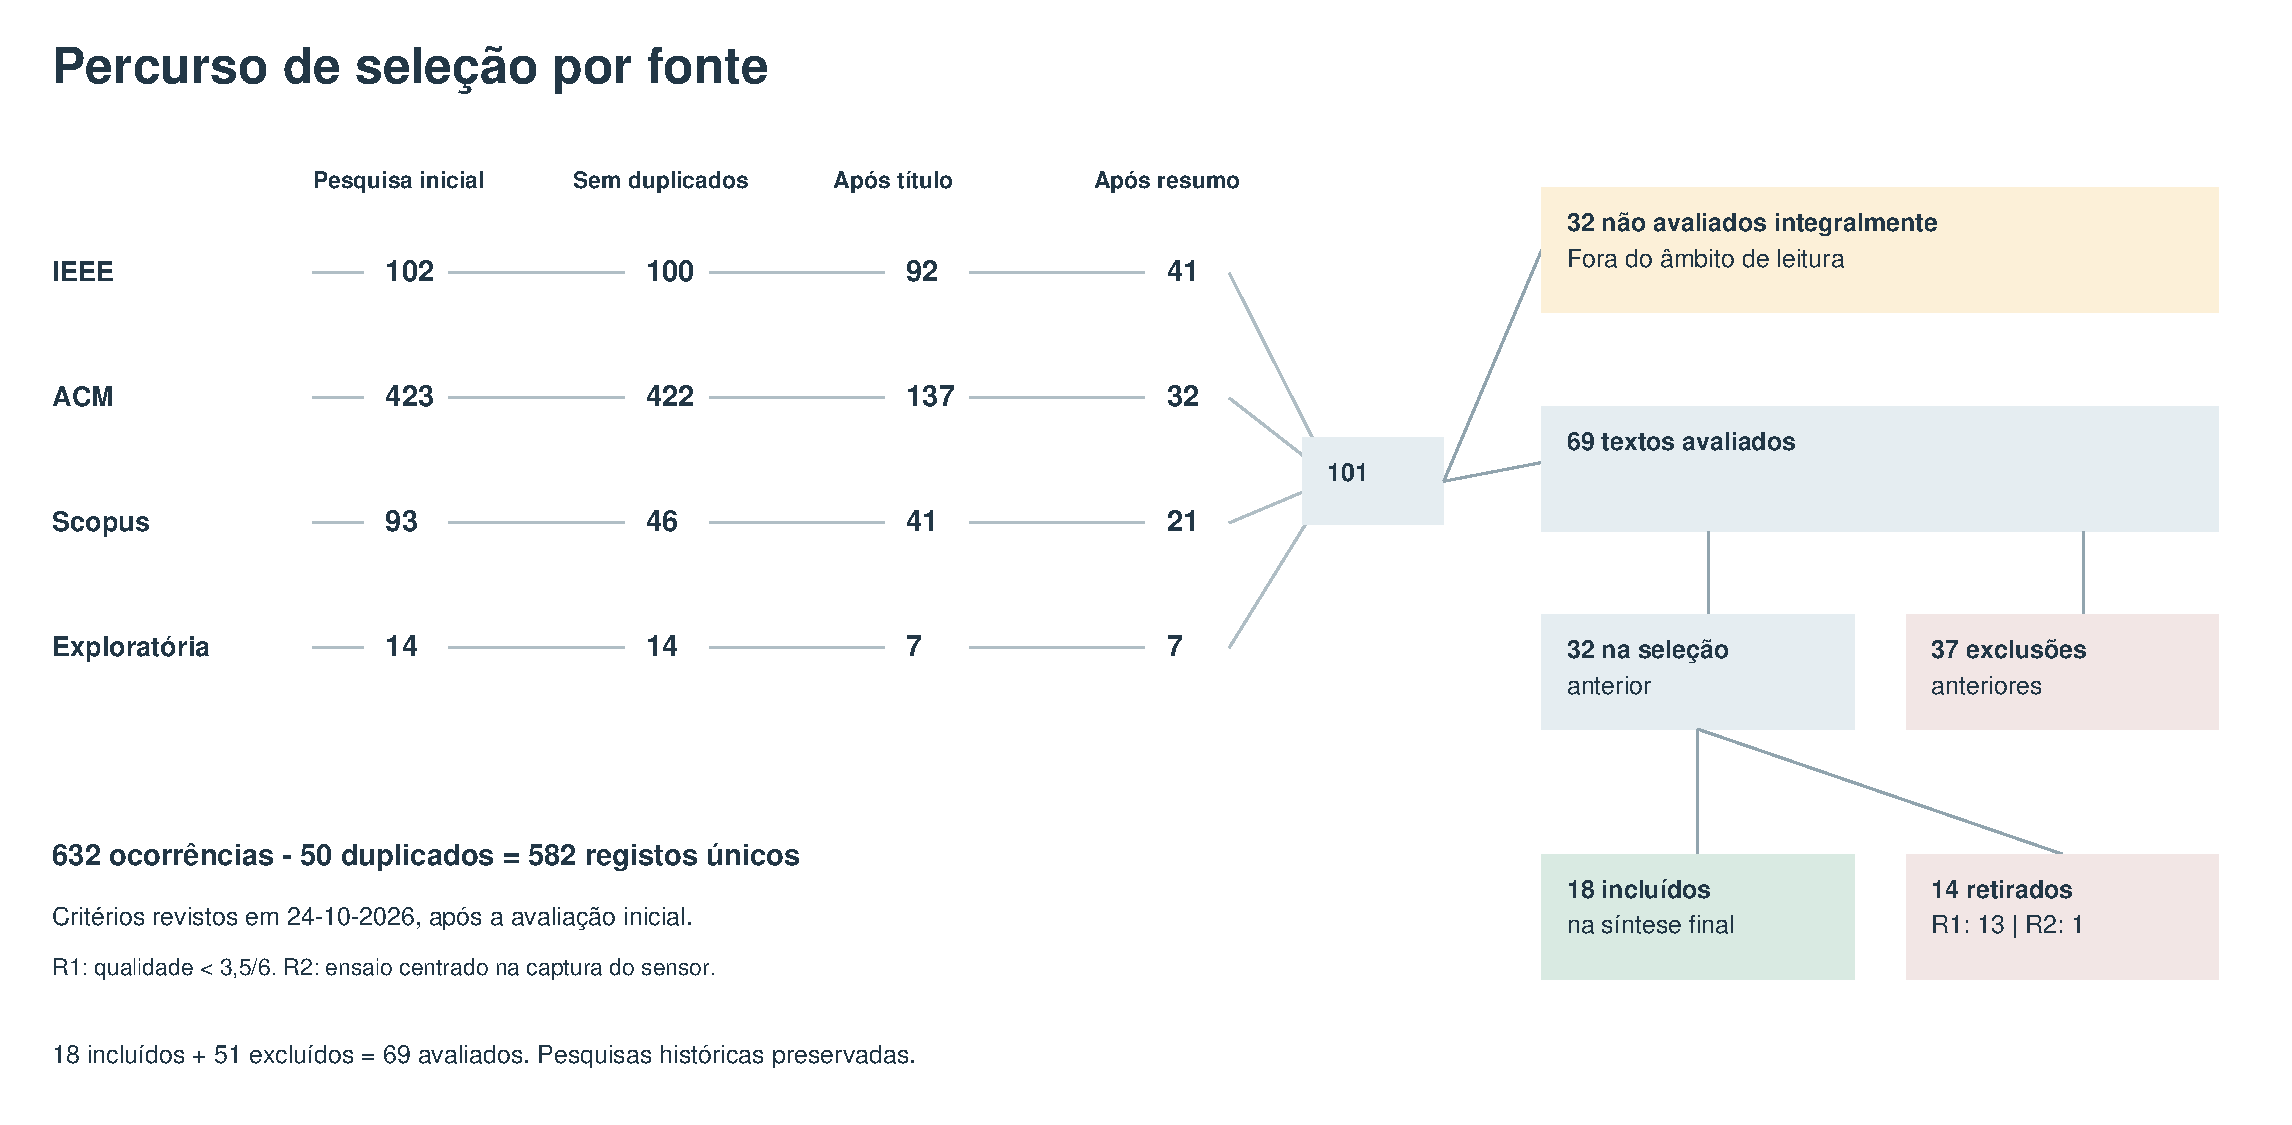
\includegraphics[width=\linewidth]{figures/fluxo-bases.pdf}
\caption[Fluxo de seleção com a etapa adicional de seleção focalizada]{Fluxo de seleção com a etapa adicional de seleção focalizada. Números derivados dos registos, sem alteração das pesquisas históricas.}\end{figure}
\begin{figure}[H]\centering
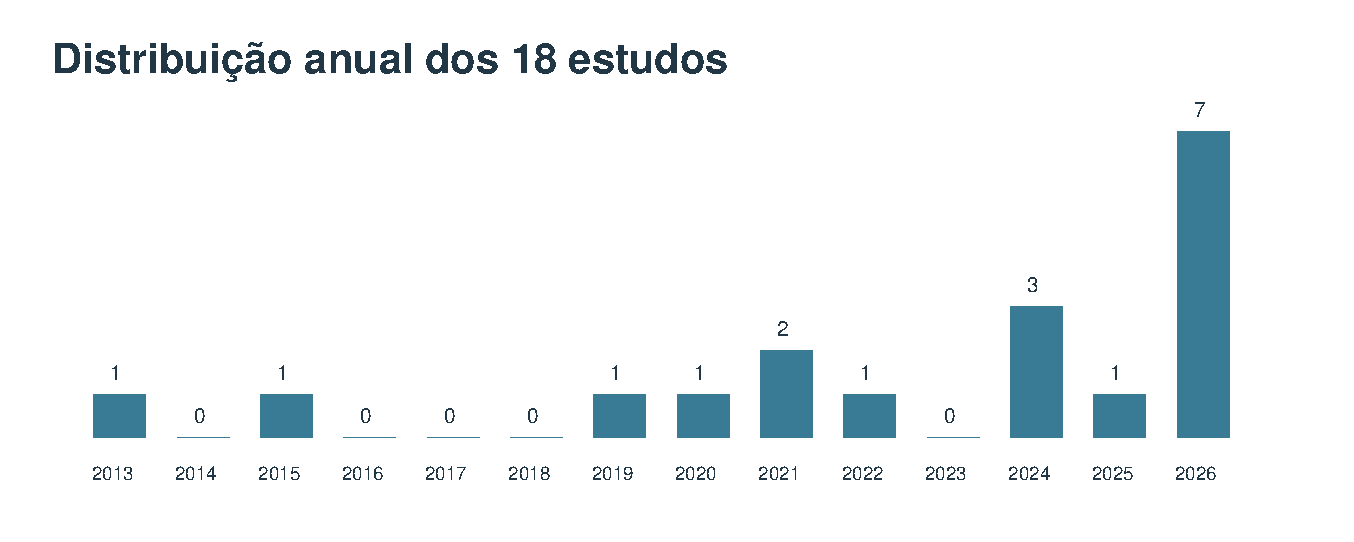
\includegraphics[width=.9\linewidth]{figures/estudos-por-ano.pdf}
\caption[Distribuição dos 18 estudos por ano]{Distribuição dos 18 estudos por ano, conferida com as referências. Cada estudo é contado uma vez; não se utiliza o gráfico anual nativo afetado pela multiplicação por respostas de qualidade.}\end{figure}

\subsection{Decisões da reformulação}
Foram reavaliados 32 estudos. A tabela seguinte identifica os 14 retirados da síntese e os respetivos motivos, preservando a avaliação anterior.
\small\begin{longtable}{@{}P{.8cm}P{8.8cm}P{1cm}P{2cm}@{}}\toprule
ID & Estudo & Q/6 & Motivo\\\midrule\endhead
P01 & Providing SIEM systems with self-adaptation & 3,0 & R1: qualidade\\
P12 & Integration of Splunk Enterprise SIEM for DDoS Attack Detection in IoT & 2,0 & R1: qualidade\\
S055 & Enhancing Cybersecurity with IDS and SIEM Integration Detection & 1,5 & R1: qualidade\\
S069 & Botnet intrusion detection: A modern architecture to defend a virtual private cloud & 2,5 & R1: qualidade\\
I001 & An Integrated Approach to AI-Enhanced Security Information and Event Management & 3,0 & R1: qualidade\\
I003 & Integrated Threat Intelligence and Event Correlation with Wazuh, Suricata, and MISP & 2,0 & R1: qualidade\\
I005 & New Types of Alert Correlation for Security Information and Event Management Systems & 1,5 & R1: qualidade\\
I008 & Hybrid NIDS Architecture Leveraging Suricata, Zeek and the ELK Stack & 3,0 & R1: qualidade\\
I009 & Intelligent Network Intrusion Detection and Prevention System (NIDPS): A Machine Learning and Network Security & 1,5 & R1: qualidade\\
I020 & Real-Time Anomaly Detection in SDN Architecture Using Integrated SIEM and Machine Learning for Enhancing Network Security & 1,5 & R1: qualidade\\
I026 & SIEM approach for a higher level of IT security in enterprise networks & 2,5 & R1: qualidade\\
I032 & Anomaly Detection in HTTP Logs: Leveraging Machine Learning for Uncovering Anomalous Traffic Patterns with SIEM Integration & 2,5 & R1: qualidade\\
I043 & Protection Against Cyber Threats by Integrating SIEM Solutions in a Demilitarized Zone: A University Network Environment as a Case Study & 2,0 & R1: qualidade\\
I062 & Advancing Snort IPS to Achieve Line Rate Traffic Processing for Effective Network Security Monitoring & 4,0 & R2: objeto do ensaio\\
\bottomrule\end{longtable}\normalsize
\subsection{Limitações de reprodução e protocolo}
As fontes principais foram IEEE (102 ocorrências), ACM (423) e Scopus (93), com 14 ocorrências exploratórias. As consultas secundárias devolveram nove registos IEEE, cinco Scopus e 374 ocorrências ACM (372 URLs distintos); não acrescentaram candidatos às pesquisas principais. A ACM secundária foi preservada por captura estruturada, não por exportação bibliográfica nativa. Os URLs históricos IEEE preservam a expressão, mas não identificam explicitamente o campo pesquisado. A consulta secundária formal não antecedeu todas as pesquisas principais.

O protocolo do docente orientou problema, pergunta, pesquisa por grupos de termos, critérios, leitura, extração e gráficos. A revisão mantém uma PI e uma síntese narrativa. A seleção posterior por qualidade, o âmbito de leitura delimitado, a ausência de validação independente e as limitações de reprodução são adaptações explicitadas; não se alega cumprimento integral de uma revisão sistemática pré-especificada. Os registos de pesquisa originais são preservados juntamente com a versão anterior de 32 estudos.
\clearpage
\subsection*{Conferência documental de 30 de outubro}
Para tornar verificáveis as condições de pesquisa, sintetizam-se abaixo os registos históricos. A pesquisa secundária acrescenta à expressão principal o grupo de termos relativos a revisões da literatura; as duas pesquisas não constituem conjuntos independentes para somar ao fluxo.
\begin{table}[H]\centering\small
\begin{tabularx}{\linewidth}{@{}P{2cm}P{2.5cm}P{2.8cm}Y@{}}\toprule
Base & Principal & Secundária & Campo e registo preservado\\\midrule
IEEE & 102; 21/10 & 9; 21/10 & Campo histórico não confirmado; exportações CSV.\\
ACM & 423; 21/10 & 374; 22/10 & Texto completo, coleção ACM; BibTeX principal e captura secundária.\\
Scopus & 93; 21/10 & 5; 22/10 & Título, resumo e palavras-chave; exportações BibTeX.\\\bottomrule
\end{tabularx}
\caption[Registo das pesquisas históricas por base]{Registo das pesquisas históricas de outubro de 2026. As consultas secundárias sobrepõem-se às principais e não são somadas ao fluxo.}
\end{table}

Na ACM, os 374 resultados capturados correspondem a 372 URLs únicos. A reconciliação de 30 de outubro encontrou correspondência bibliográfica para os 372 na exportação nativa principal. O subconjunto BibTeX e a correspondência entre URL capturado e chave bibliográfica foram conservados nos registos de trabalho disponíveis no repositório. Trata-se de uma reconstrução documental a partir dos ficheiros originais, não de uma exportação nativa da consulta secundária nem de uma nova pesquisa. Esta reconciliação recupera as citações e confirma a sobreposição, preservando as contagens históricas.

No IEEE, executou-se em 30 de outubro uma consulta de validação com os três grupos da expressão principal e o campo \textit{All Metadata} explícito em cada termo, sem filtros adicionais. Foram apresentados 105 resultados. A expressão e o URL ficaram registados na documentação de trabalho disponível no repositório; a exportação bibliográfica obtida abrange apenas 30 resultados, não a totalidade da consulta. Esta verificação documenta uma configuração atual reproduzível, mas não demonstra qual foi o campo efetivo da pesquisa histórica. Os 105 resultados não foram incorporados na seleção nem substituem os 102 do fluxo original: o corpus desta entrega permanece fechado nos 18 estudos.

A conferência do protocolo distingue o que está concluído do que é uma adaptação: problema e pergunta única, PICOC, expressões, critérios, fluxo, leitura e extração dos 18 incluídos estão documentados. A consulta secundária formal posterior a parte das pesquisas, a leitura integral delimitada e a reformulação posterior dos critérios permanecem limitações. Não se convertem essas diferenças em etapas retroativamente cumpridas. Os 180 campos de extração foram confrontados com o Parsifal e os 18 formulários encontram-se concluídos.

\clearpage
\section{Capturas dos gráficos do Parsifal}\label{app:parsifal}
As capturas seguintes documentam os gráficos nativos da revisão. As contagens de importação incluem duplicados e registos não incluídos na síntese; a seleção final mantém 18 estudos. A distribuição anual utilizada neste relatório é a figura corrigida do apêndice anterior, com contagem única por estudo.

\begin{figure}[H]\centering
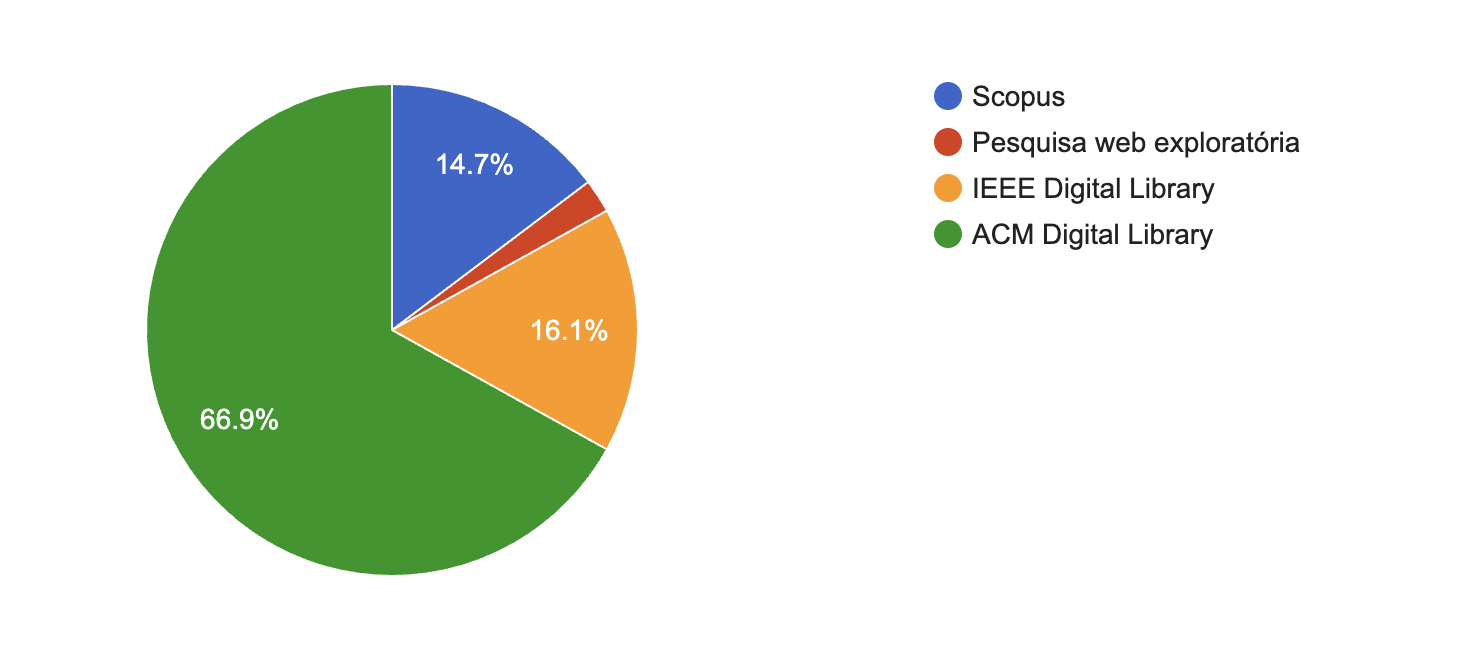
\includegraphics[width=\linewidth]{imagens/parsifal-fontes.png}
\caption[Registos importados por fonte no Parsifal]{Distribuição dos 632 registos importados por fonte, antes da deduplicação e da seleção: ACM, 423 (66,9\%); IEEE, 102 (16,1\%); Scopus, 93 (14,7\%); pesquisa exploratória, 14 (2,2\%). As percentagens são arredondadas e não representam a distribuição dos 18 estudos incluídos. Fonte: captura do Parsifal fornecida pelo grupo.}\label{fig:parsifal-fontes}
\end{figure}

\begin{figure}[H]\centering
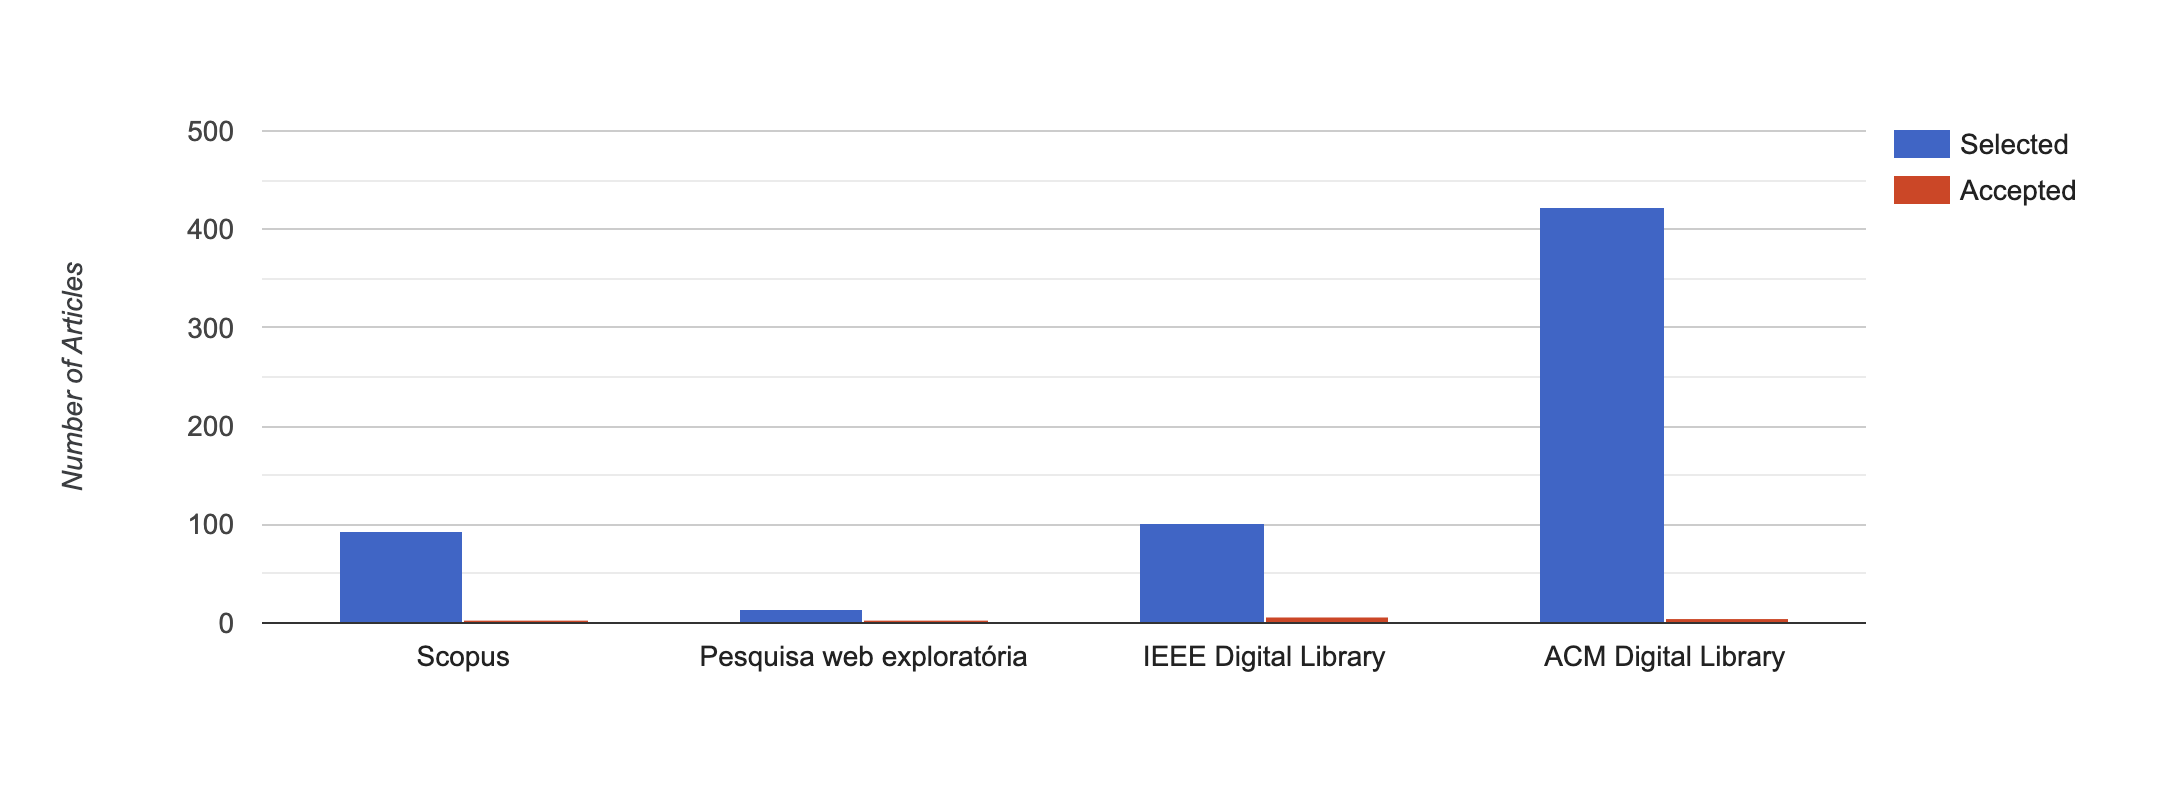
\includegraphics[width=\linewidth]{imagens/parsifal-selecao.png}
\caption[Registos importados e estudos aceites no Parsifal]{Comparação por fonte no Parsifal. A série azul, designada \textit{Selected} pela aplicação, representa os registos importados: Scopus, 93; exploratória, 14; IEEE, 102; ACM, 423. A série vermelha, \textit{Accepted}, representa os 18 estudos aceites: 3, 3, 7 e 5, respetivamente. A escala comum torna as barras dos aceites pouco visíveis; a figura de incluídos no corpo do relatório apresenta esses valores separadamente. Fonte: captura do Parsifal fornecida pelo grupo.}\label{fig:parsifal-selecao}
\end{figure}

\clearpage
\phantomsection
\addcontentsline{toc}{section}{\refname}
\bibliographystyle{unsrtnat}
\bibliography{references}
\end{document}
